% !TEX encoding = UTF-8 Unicode
\documentclass[a4paper]{article}

\usepackage[utf8]{inputenc}
\usepackage{erk}
\usepackage{times}
\usepackage{graphicx}
\usepackage{cite}
\usepackage{array}
\usepackage[top=22.5mm, bottom=22.5mm, left=22.5mm, right=22.5mm]{geometry}

\usepackage[english]{babel}

% local definitions
\def\footnotemark{}%  to avoid footnote on cover page

\begin{document}
%make title
\title{New dataset of emotional and color responses to music}

\author{Primož Godec$^{1}$, Matevž Pesek$^{1}$, Mojca Poredoš$^{1}$, Gregor Strle$^{2}$,\\ Jože Guna$^{3}$, Emilija Stojmenova$^{3}$, Matevž Pogačnik$^{3}$ and Matija Marolt$^{1}$} % use ^1, ^2 for author(s) from different institutions

\affiliation{$^{1}$University of Ljubljana, Faculty of computer and information science \\ 
$^{2}$Institute of Ethnomusicology, Scientfic Research Centre of the Slovenian Academy of Sciences and Arts \\
$^{3}$University of Ljubljana, Faculty of Electrotechnics}

\email{E-mail: \{matevz.pesek, matija.marolt\}@fri.uni-lj.si, \{primoz.godec, mojca.poredos\}@lgm.fri.uni-lj.si \\ gregor.strle@zrc-sazu.si,  \{joze.guna, emilija.stojmenova, matevz.pogacnik\}@fe.uni-lj.si}

\maketitle

\begin{abstract}{Abstract}
This paper presents a new dataset gathered containing perceived and induced emotions for 200 audio clips. The gathered dataset also provides users' association of color for each clip, along with users' demographic and personal data, such as users' emotion state, preferred genres, music experience and daily inference, and others. With an online survey we collected more than 7000 responses for a dataset of 200 audio excerpts, thus providing about 37 user responses per clip. We introduced a new methodology for gathering user perception of emotions in a form of two new interfaces - the MoodGraph and MoodStripe. We present a preliminary evaluation of classifying the present emotions with a regression algorithm on the gathered dataset, and perform a comparison towards other datasets and algorithms.
\end{abstract}

\section{Introduction}

The intention of this study is to provide a dataset for the research in a highly subjective field of multi-modal perception and the connecting relations between the music, colors and emotions. The problem has been previously well formalised in the field of psychology; however, it is our intention to tackle the problem in the domain of signal processing. In order to achieve the desired goal, we gathered a dataset possibly covering several aspects such as personal information, current mood state of the user and his music taste and experience. Many researchers have worked on similar problems; however, there are several undiscovered relations that brought the problem to our attention. Music mood from year to year has become very important field in music information retrieval. Several machine learning algorithms have been made for mood estimation from audio. Schmidt et al. \cite{schmidt2009projection} uses regression for mood classification. Panda et al. use support vector machines \cite{ben2010user}, k-nearest neighbors, C4.5 and naive bayes. Support vector machine was also used by \cite{laurier2007audio}. Barthet et al. uses Support vector regression for classification.
MIREX (Music Information Retrieval Evaluation eXchange) organises mood classification task from 2007. 

These algorithm can be used in music recommendation systems based on mood. Because we plan to make music recommendation system, we decided to make research of music mood. The beginning of our research was to gather new dataset on which we have building our research.

Several datasets were gathered in past and some of them were available online. Eerola et al \cite{eerola2010comparison} performed a gathering of the film music dataset. Sound track for music and emotions provides single mean rating with label and values in three-dimensional model. Dataset contains values for 361 film music clips.  The Mood Swings Turk Dataset contains average 17 valence-arousal ratings for 240 audio clips \cite{schmidt2011modeling}. Clips in this dataset are of popular music. The Cal500 provides mood labels for 500 western popular songs \cite{turnbull2008semantic}. They have around 3 annotations per song. MTV Music Dataset contains 5 bipolar valence-arousal ratings for 192 popular songs \cite{schuller2010mister}. Songs were selected between songs MTV has played on his channel.

This collections of datasets we want to add our new dataset for 200 audio clips. We not only wanted to gather huge dataset, but also dataset a lot of user responses. In addition to responses on music clips, we collected some other participant's demographic data and perception of mood. This data might help us to understand difference in responses to audio clips.

In order to evaluate the usefulness of the collected data and possibly highlight the importance of the relations between the modalities and the user's personal data, we performed a preliminary evaluation of the mood estimation algorithm using the regression for valence-arousal prediction, as described in \cite{schmidt2009projection}. This algorithm was tested on our dataset and Mood Swing Turk dataset \cite{schmidt2011modeling}.

The paper is structured as follows: section 2 describes the survey and it design, section 3 provides analyses of the gathered data and survey evaluation and section 4 concludes the paper and describes our future work.


\section{Online survey}

Online survey was used for data gathering. Before our survey was made, decision about choosing mood labels had made. Some basic emotion labels exist \cite{dalgleish1999handbook}, but there is no standard set in music and mood research. Others choose label sets intuitively, without any explanations \cite{wu2013spectral}. In order to use an optimal set of labels, we prepared preliminary survey 

This survey has two parts. In first we prepared some basic demographical questions and questions about user perception of mood. We test basic structure and questions type of main survey. But the most important was second part. Participants were asked describe his emotional state on scale from 1 to 7 for each of 48 emotional labels. We also test response on continuous color wheel used to describe connection between mood and colors. 

Depending on results of this questionnaire we selected 17 basic emotion labels which strongly correlate to three basic components that explain 64\% of the variance to the dataset. Depending on user responses and results we also decided to restrict continuous color wheel on that with 49 colors. 

\subsection{The survey}

We structured our survey in three sections. We captured user personal characteristic in first part. User was asked to answer on some demographical questions: age, area of living and native language. Some data about users music education, listening to the music and genre preference was captured. We did not want to be too long with this part, but we think that it is important to have that type of data, because this help us to understand users mood perception. For example we think that users who like metal, marked that that type of music is more positive, than other users.

Second part contains questions about user perceptions of mood and connection between color and mood. First we asked for user current mood state with three different tasks. User had place his current mood in valence arousal space. It is 2D plane to describe pleasantness and activeness of the mood. Then we wanted to know user's perception of current mood by selecting color. User also had to mark how strong one emotional state is expressed in him. It was captured with new element we described in \cite{pesek2014gathering} named MoodStripe (Figure \ref{moodstripe}). Second part has also two tasks that directly capture music mood perception. First participant was asked to place 10 emotional labels in valence-arousal space described before. For this part we used self designed element named MoodGraph (Figure \ref{moodgraph}). Then they were asked to choose color that best match to labels used before. That part tells us user perception of mood labels, that was also used in third part of our survey. 

\begin{figure}[ht]
\centering
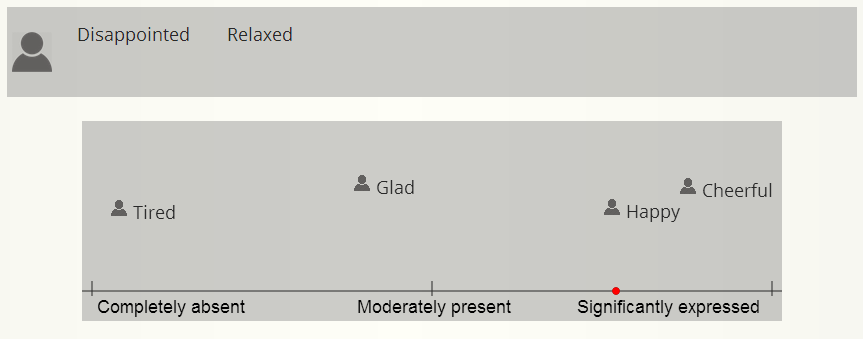
\includegraphics[width=80mm]{moodstripe.png}
\caption{New element used in our survey named MoodStripe. With drag and drop technique user place emotion labels in plane depending on how is emotion expressed. When place on left this mean that emotion is totally absent, when placed on right mean that emotion is significantly  expressed. }
\label{moodgraph}
\end{figure}

\begin{figure}[ht]
\centering
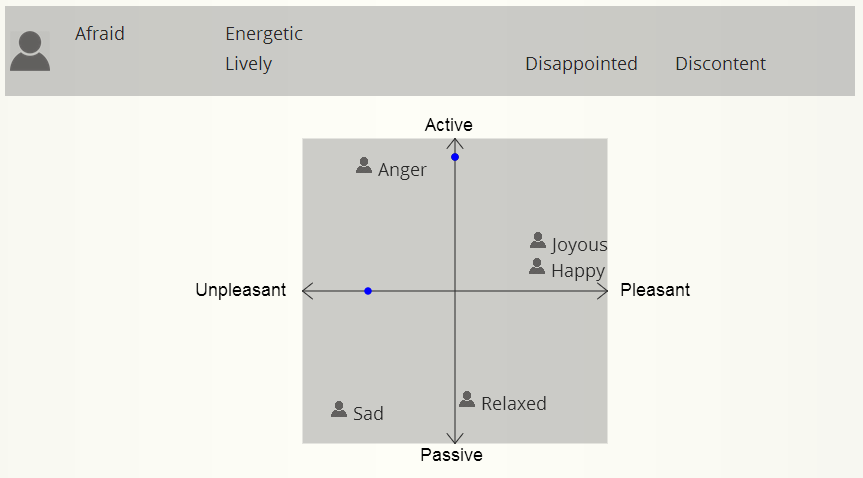
\includegraphics[width=80mm]{moodgraph.png}
\caption{New element used in our survey named MoodGraph. With it we capture pleasantness on x axis and activeness on y axis. }
\label{moodgraph}
\end{figure}

In last part of our survey user was asked to make two actions for each of 10 audio clips. Clips are 15 second long and was randomly selected from base of 200 clips. All selected audio clips are for most of users unknown, to avoid bias because of familiarity of song. We gathered music from four sources. Eighty songs was chosen from the free online music service Jamendo. We selected songs from as many genre as possible. Next 80 clips was from film music dataset and is described here \cite{eerola2010comparison}. We also provide 20 clips from collection of slovenian folk music collection and 20 of the contemporary electro-acoustic music collection. 

For each clip we asked user to select color, that he think best describes music clip. User was also asked select emotion labels that best describe clip and place them in valence-arousal space. We provide two group of labels. From first group user select emotions that was induced by song in music and from second emotions perceived in song.

\section{Results}

\begin{table*}[t]
\caption{Results in prediction valence arousal using regression}
\\
\begin{tabular}{| l | c | c | c | c | c | c |}
\hline
Feature & Avg. distance & Near. distance & Avg. dist in sdt & Avg. distance & Near. distance & Avg. dist in sdt \\
\hline
MFCC & 0.2060 & 0.0595 & 0.4870 & 0.2448 & 0.0641 & 0.6514\\
Chroma & 0.2215 & 0.0614 & 0.4993 & 0.3316 & 0.1026 & 0.8940\\
\hline
\end{tabular}
\label{regressionresults}
\end{table*}

We got 7187 responses from 1357 persons in our survey. Dataset contains 200 audio clips. It means that we have average 37 responses per audio clip. There is no mood-music dataset with such ratio per clip as we know. Each of these responses contains at least one labels that participant selected as induced and labels that participants select as perceived in audio. User was selecting between 10 labels for induced and between 14 labels for perceived and place it in valence-arousal space using MoodGraph (Figure \ref{moodgraph}). Each response also contains color participants think best describe audio clip. 

For each user we also gathered some demographical data, data about music education, data about listening music and perception of music-mood. Dataset will be published when we finish with second part of survey. We will show short demographical analysis in next part. With  data gathered we also trained regression algorithm, result will be shown in following subsections. 

\subsection{Demographic analysis}

Average participant age are 26.5 years. Youngest is 15, oldest is 64 years old. 65\% of participants are women. One third of participants are from urban area. 50\% of participants have musical education and 53\% of participants play instrument or sing. Most of participants (30\%) listen to the music average from 1 to 2 hours per day. 3\% of participants admit that they were under influence of drugs when taking survey.

\subsection{Predicting valence-arousal values using regression}

Finally we tested our data on one of algorithms for evaluating mood from music. We implemented regression algorithm used in \cite{schmidt2009projection}. We used least squares method on MFCC \cite{logan2000mel} and Chroma \cite{bello2005robust}  features. MFCCs was calculated with cepstral coefficients 20, Chroma was calculated using 12 bins. First features was calculated using LibROSA python library on a 15 seconds audio clips from dataset. Dataset was divided in 2 parts. First set contains 70\% of dataset and was used for training algorithm using least squares \cite{abdi2007method}. Training was made with mean values of valence and arousal. This algorithm returns vector $b$ as result. Second set (containing other 30\% of dataset) was used to test valence and arousal prediction. Values was calculated separately for valence and arousal using following equation: $$y = X b$$ where $X$ is feature matrix. Each row represents one vector of features for audio clip. $b$ is vector calculated with regression algorithm and maps values from feature space to valence or arousal value. $y$ is vector of predictions for valence or arousal. 

\begin{figure}[ht]
\centering
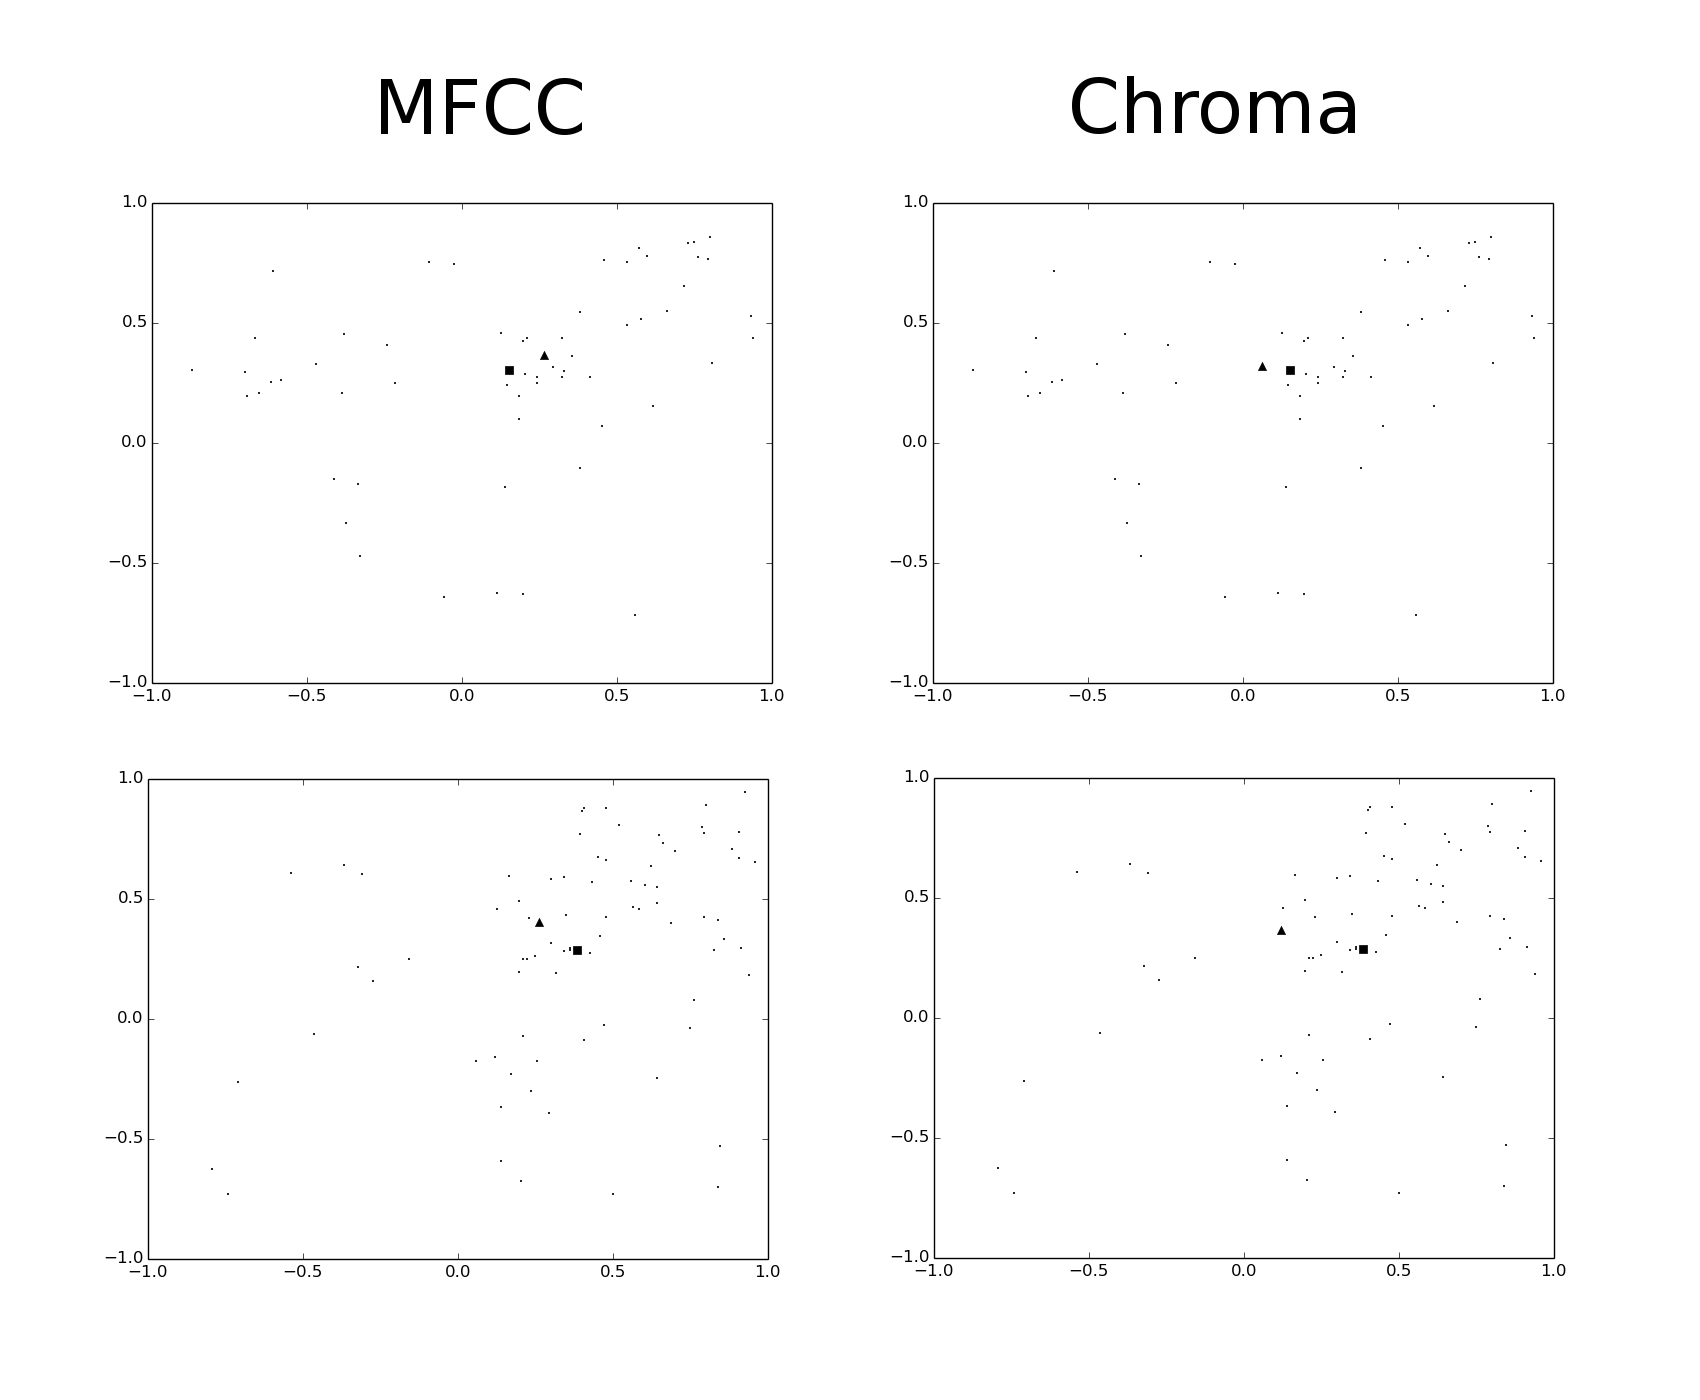
\includegraphics[width=80mm]{graphs.png}
\caption{Image shows 4 valence-arousal spaces, where raises pleasantness from left to right on x axis and activeness fro bottom to top on z axis. First row shows prediction on songs with id 413 using MFCC and Chroma. Same is shown for song 571 in second row. Triangle shows regression algorithm prediction, square shows mean value of all valence-arousal values gathered with survey. Dots show all valence-arousal values gathered.  }
\label{graphs}
\end{figure}

Results using regression algorithm are shown in table \ref{regressionresults}. For regression with MFCC and regression with Chroma average distance between estimated and mean valence-arousal value was calculated. We also provide average distance to nearest value in dataset and the average distance between the mean valence-arousal point and the prediction, measured in the size of the standard deviation of data. Same algorithm was also used on features Schmidt et al. provides for Mood Swing dataset \cite{schmidt2011modeling} to compare results. 

Our results shows that there is better correlation between MFCC and valence-arousal than this between Chroma and valence arousal. From table is also seen that we got better result on our dataset than results on Mood Swing dataset are.  

\newcolumntype{L}[1]{>{\raggedright\arraybackslash}p{#1}}
\newcolumntype{C}[1]{>{\centering\arraybackslash}p{#1}}
\newcolumntype{R}[1]{>{\raggedleft\arraybackslash}p{#1}}

\begin{table}[h]
\caption{Average distances between predictions and mean valence-arousal value separately for valence and arousal}
\begin{tabular}{|L{2cm}|C{2.2cm}|C{2.2cm}|}
\hline
 & MFCC & Chroma \\
\hline
Valence & 0.1734 & 0.1826 \\
Arousal & 0.0871 & 0.0940 \\
\hline
\end{tabular}
\label{seperateresults}
\end{table}

Table \ref{seperateresults} shows accuracy in predictions separately for valence and arousal values measured in average distance between prediction and mean valence-arousal value from dataset. Result shows that with prediction used regression method are better for arousal component. That means that there is better correlation between booth features and arousal than between features and valence. 

\section{Future work and conclusion}

We gathered well annotated dataset with a lot of responses with online survey, which will be public soon as possible. It contains some users demographical data, users mood and color perception and the most important a lot of mood and color responses for audio clips dataset. Each of this responses contains induced emotions and perceived emotions with valence-arousal values. It also contains color perception for audio. Unlike many others datasets our will also provide audio clips used in survey. 

This dataset open new possibilities for research mood evaluation from audio. Mood evaluation is important for music recommendation systems based on mood. Personal data in our dataset provide possibilities to research usefulness of this data in music recommendation. Our dataset also provides better results in regression in comparison with other datasets.

Shortly we will begin with second run of survey. This survey will be in english language and will contains more audio clips. With second run we want to raise number of responses per clip and enlarge number of audio clips in dataset. We will continue testing mood evaluation algorithms on dataset and compare with results on other datasets. Then we will make our own classification algorithm. We plan that our algorithm will not only use audio features like other known algorithms, but also data that describes users perception of mood.

We will explore correlation between mood and colors. If results are useful, it will be used for music visualisation. Visualisation will be used in music recommendation interface, we plan to develop. It will be using our mood evaluation algorithm. 

Our dataset will be also used in research and also available to other researchers online and free for use. 

\bibliography{erkbib}{}

\bibliographystyle{plain}

\end{document}
